\subsubsection{Alarms}

\begin{center}
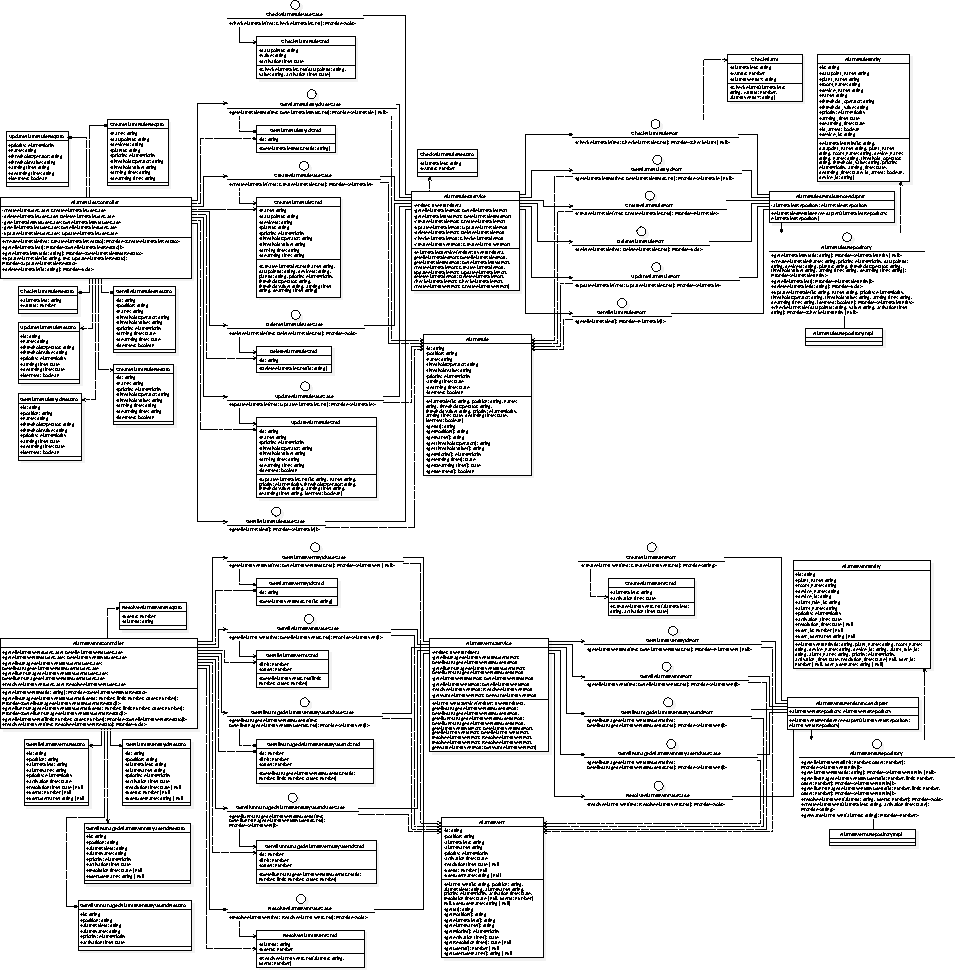
\includegraphics[width=\textwidth]{./backend/alarms/alarms.pdf}
\captionof{figure}{Diagramma delle classi del modulo Alarms}
\end{center}

% req dto

\addAtr{}{name: string}{Nome della regola di allarme}
\addAtr{}{datapointId: string}{Identificativo del datapoint monitorato}
\addAtr{}{deviceId: string}{Identificativo del dispositivo associato}
\addAtr{}{plantId: string}{Identificativo dell'impianto associato}
\addAtr{}{priority: AlarmPriority}{Livello di priorità dell'allarme}
\addAtr{}{thresholdOperator: string}{Operatore di confronto per la soglia (es. >, <, =)}
\addAtr{}{thresholdValue: string}{Valore soglia che determina l'attivazione dell'allarme}
\addAtr{}{armingTime: string}{Orario di attivazione della regola di allarme}
\addAtr{}{dearmingTime: string}{Orario di disattivazione della regola di allarme}
\makeCl{CreateAlarmRuleReqDto}{DTO di richiesta per la creazione di una nuova regola di allarme}

\addAtr{}{userId: number}{Identificativo dell'utente che risolve l'evento}
\addAtr{}{alarmId: string}{Identificativo dell'evento di allarme da risolvere}
\makeCl{ResolveAlarmEventReqDto}{DTO di richiesta per la risoluzione di un evento di allarme}

\addAtr{}{priority: AlarmPriority}{Nuovo livello di priorità dell'allarme}
\addAtr{}{name: string}{Nuovo nome della regola di allarme}
\addAtr{}{thresholdOperator: string}{Nuovo operatore di confronto per la soglia}
\addAtr{}{thresholdValue: string}{Nuovo valore soglia}
\addAtr{}{armingTime: string}{Nuovo orario di attivazione}
\addAtr{}{dearmingTime: string}{Nuovo orario di disattivazione}
\addAtr{}{isArmed: boolean}{Indica se la regola è attualmente armata}
\makeCl{UpdateAlarmRuleReqDto}{DTO di richiesta per l'aggiornamento di una regola di allarme esistente}

% res dto

\addAtr{}{alarmRuleId: string}{Identificativo della regola di allarme verificata}
\addAtr{}{wardId: number}{Identificativo del ward associato alla regola}
\makeCl{CheckAlarmRuleResDto}{DTO di risposta per la verifica di una regola di allarme}

\addAtr{}{id: string}{Identificativo univoco della regola creata}
\addAtr{}{name: string}{Nome della regola di allarme creata}
\addAtr{}{priority: AlarmPriority}{Priorità assegnata alla regola}
\addAtr{}{thresholdOperator: string}{Operatore di confronto della soglia}
\addAtr{}{thresholdValue: string}{Valore soglia configurato}
\addAtr{}{armingTime: string}{Orario di attivazione configurato}
\addAtr{}{dearmingTime: string}{Orario di disattivazione configurato}
\addAtr{}{isArmed: boolean}{Stato di armamento iniziale della regola}
\makeCl{CreateAlarmRuleResDto}{DTO di risposta restituito dopo la creazione di una regola di allarme}

\addAtr{}{id: string}{Identificativo univoco dell'evento di allarme}
\addAtr{}{position: string}{Posizione fisica del dispositivo che ha generato l'evento}
\addAtr{}{alarmRuleId: string}{Identificativo della regola che ha generato l'evento}
\addAtr{}{alarmName: string}{Nome dell'allarme associato all'evento}
\addAtr{}{priority: AlarmPriority}{Priorità dell'evento di allarme}
\addAtr{}{activationTime: Date}{Timestamp di attivazione dell'evento}
\addAtr{}{resolutionTime: Date $|$ null}{Timestamp di risoluzione, null se non ancora risolto}
\addAtr{}{userId: number $|$ null}{Identificativo dell'utente che ha risolto l'evento, null se non risolto}
\addAtr{}{userUsername: string $|$ null}{Username dell'utente che ha risolto l'evento, null se non risolto}
\makeCl{GetAlarmEventByIdResDto}{DTO di risposta contenente i dettagli di un singolo evento di allarme}

\addAtr{}{id: string}{Identificativo univoco della regola di allarme}
\addAtr{}{position: string}{Posizione fisica del dispositivo monitorato}
\addAtr{}{name: string}{Nome della regola di allarme}
\addAtr{}{thresholdOperator: string}{Operatore di confronto della soglia}
\addAtr{}{thresholdValue: string}{Valore soglia configurato}
\addAtr{}{priority: AlarmPriority}{Priorità della regola}
\addAtr{}{armingTime: Date}{Orario di attivazione della regola}
\addAtr{}{dearmingTime: Date}{Orario di disattivazione della regola}
\addAtr{}{isArmed: boolean}{Indica se la regola è attualmente armata}
\makeCl{GetAlarmRuleByIdResDto}{DTO di risposta contenente i dettagli di una singola regola di allarme}

\addAtr{}{id: string}{Identificativo univoco dell'evento}
\addAtr{}{position: string}{Posizione fisica del dispositivo che ha generato l'evento}
\addAtr{}{alarmRuleId: string}{Identificativo della regola associata}
\addAtr{}{alarmName: string}{Nome dell'allarme associato}
\addAtr{}{priority: AlarmPriority}{Priorità dell'evento}
\addAtr{}{activationTime: Date}{Timestamp di attivazione}
\addAtr{}{resolutionTime: Date $|$ null}{Timestamp di risoluzione, null se non ancora risolto}
\addAtr{}{userId: number $|$ null}{Identificativo dell'utente che ha risolto l'evento}
\addAtr{}{userUsername: string $|$ null}{Username dell'utente che ha risolto l'evento}
\makeCl{GetAllAlarmEventsResDto}{DTO di risposta per un elemento della lista di tutti gli eventi di allarme}

\addAtr{}{id: string}{Identificativo univoco della regola}
\addAtr{}{position: string}{Posizione fisica del dispositivo monitorato}
\addAtr{}{name: string}{Nome della regola di allarme}
\addAtr{}{thresholdOperator: string}{Operatore di confronto della soglia}
\addAtr{}{thresholdValue: string}{Valore soglia configurato}
\addAtr{}{priority: AlarmPriority}{Priorità della regola}
\addAtr{}{armingTime: Date}{Orario di attivazione}
\addAtr{}{dearmingTime: Date}{Orario di disattivazione}
\addAtr{}{isArmed: boolean}{Indica se la regola è attualmente armata}
\makeCl{GetAllAlarmRulesResDto}{DTO di risposta per un elemento della lista di tutte le regole di allarme}

\addAtr{}{id: string}{Identificativo univoco dell'evento}
\addAtr{}{position: string}{Posizione fisica del dispositivo}
\addAtr{}{alarmRuleId: string}{Identificativo della regola associata}
\addAtr{}{alarmName: string}{Nome dell'allarme}
\addAtr{}{priority: AlarmPriority}{Priorità dell'evento}
\addAtr{}{activationTime: Date}{Timestamp di attivazione}
\addAtr{}{resolutionTime: Date $|$ null}{Timestamp di risoluzione, null se non ancora risolto}
\addAtr{}{userUsername: string $|$ null}{Username dell'utente che ha gestito l'evento}
\makeCl{GetAllManagedAlarmEventsByUserIdResDto}{DTO di risposta per un elemento della lista degli eventi gestiti da un utente specifico}

\addAtr{}{id: string}{Identificativo univoco dell'evento}
\addAtr{}{position: string}{Posizione fisica del dispositivo}
\addAtr{}{alarmRuleId: string}{Identificativo della regola associata}
\addAtr{}{alarmName: string}{Nome dell'allarme}
\addAtr{}{priority: AlarmPriority}{Priorità dell'evento}
\addAtr{}{activationTime: Date}{Timestamp di attivazione}
\makeCl{GetAllUnmanagedAlarmEventsByUserIdResDto}{DTO di risposta per un elemento della lista degli eventi non ancora gestiti assegnati a un utente}

\addAtr{}{id: string}{Identificativo univoco della regola aggiornata}
\addAtr{}{name: string}{Nome aggiornato della regola}
\addAtr{}{thresholdOperator: string}{Operatore di confronto aggiornato}
\addAtr{}{thresholdValue: string}{Valore soglia aggiornato}
\addAtr{}{priority: AlarmPriority}{Priorità aggiornata}
\addAtr{}{armingTime: Date}{Orario di attivazione aggiornato}
\addAtr{}{dearmingTime: Date}{Orario di disattivazione aggiornato}
\addAtr{}{isArmed: boolean}{Stato di armamento aggiornato}
\makeCl{UpdateAlarmRuleResDto}{DTO di risposta restituito dopo l'aggiornamento di una regola di allarme}

% model

\addAtr{-}{id: string}{Identificativo univoco dell'evento di allarme}
\addAtr{-}{position: string}{Posizione fisica del dispositivo che ha generato l'evento}
\addAtr{-}{alarmRuleId: string}{Identificativo della regola che ha generato l'evento}
\addAtr{-}{alarmName: string}{Nome dell'allarme associato}
\addAtr{-}{priority: AlarmPriority}{Priorità dell'evento}
\addAtr{-}{activationTime: Date}{Timestamp di attivazione dell'evento}
\addAtr{-}{resolutionTime: Date $|$ null}{Timestamp di risoluzione, null se non ancora risolto}
\addAtr{-}{userId: number $|$ null}{Identificativo dell'utente che ha risolto l'evento}
\addAtr{-}{userUsername: string $|$ null}{Username dell'utente che ha risolto l'evento}
\addMet{+}{getId(): string}{Restituisce l'identificativo univoco dell'evento}
\addMet{+}{getPosition(): string}{Restituisce la posizione del dispositivo}
\addMet{+}{getAlarmRuleId(): string}{Restituisce l'identificativo della regola associata}
\addMet{+}{getAlarmName(): string}{Restituisce il nome dell'allarme}
\addMet{+}{getPriority(): AlarmPriority}{Restituisce la priorità dell'evento}
\addMet{+}{getActivationTime(): Date}{Restituisce il timestamp di attivazione}
\addMet{+}{getResolutionTime(): Date $|$ null}{Restituisce il timestamp di risoluzione}
\addMet{+}{getUserId(): number $|$ null}{Restituisce l'identificativo dell'utente risolutore}
\addMet{+}{getUserUsername(): string $|$ null}{Restituisce lo username dell'utente risolutore}
\makeCl{AlarmEvent}{Modello di dominio che rappresenta un evento di allarme generato da una regola}

\addAtr{-}{id: string}{Identificativo univoco della regola di allarme}
\addAtr{-}{position: string}{Posizione fisica del dispositivo monitorato}
\addAtr{-}{name: string}{Nome della regola di allarme}
\addAtr{-}{thresholdOperator: string}{Operatore di confronto usato per valutare la soglia}
\addAtr{-}{thresholdValue: string}{Valore soglia configurato per l'attivazione}
\addAtr{-}{priority: AlarmPriority}{Livello di priorità della regola}
\addAtr{-}{armingTime: Date}{Orario a partire dal quale la regola è attiva}
\addAtr{-}{dearmingTime: Date}{Orario a partire dal quale la regola è inattiva}
\addAtr{-}{isArmed: boolean}{Indica se la regola è attualmente in stato armato}
\addMet{+}{getId(): string}{Restituisce l'identificativo univoco della regola}
\addMet{+}{getPosition(): string}{Restituisce la posizione del dispositivo monitorato}
\addMet{+}{getName(): string}{Restituisce il nome della regola}
\addMet{+}{getThresholdOperator(): string}{Restituisce l'operatore di confronto della soglia}
\addMet{+}{getThresholdValue(): string}{Restituisce il valore soglia}
\addMet{+}{getPriority(): AlarmPriority}{Restituisce la priorità della regola}
\addMet{+}{getArmingTime(): Date}{Restituisce l'orario di attivazione}
\addMet{+}{getDearmingTime(): Date}{Restituisce l'orario di disattivazione}
\addMet{+}{getIsArmed(): boolean}{Restituisce lo stato di armamento della regola}
\makeCl{AlarmRule}{Modello di dominio che rappresenta una regola di allarme configurabile}

\addAtr{+}{alarmRuleId: string}{Identificativo della regola di allarme verificata}
\addAtr{+}{wardId: number}{Identificativo del ward associato alla regola}
\makeCl{CheckAlarm}{Oggetto di dominio risultante dalla verifica di una regola di allarme}

% controller

\addAtr{-}{getAllAlarmEventsUseCase: GetAllAlarmEventsUseCase}{Use case per il recupero di tutti gli eventi di allarme}
\addAtr{-}{getAlarmEventByIdUseCase: GetAlarmEventByIdUseCase}{Use case per il recupero di un evento per identificativo}
\addAtr{-}{getAllManagedAlarmEventsByUserIdUseCase: GetAllManagedAlarmEventsByUserIdUseCase}{Use case per il recupero degli eventi gestiti da un utente}
\addAtr{-}{getAllUnmanagedAlarmEventsByUserIdUseCase: GetAllUnmanagedAlarmEventsByUserIdUseCase}{Use case per il recupero degli eventi non gestiti assegnati a un utente}
\addAtr{-}{resolveAlarmEventUseCase: ResolveAlarmEventUseCase}{Use case per la risoluzione di un evento di allarme}
\addMet{+}{getAlarmEventById(id: string): Promise$<$GetAlarmEventByIdResDto$>$}{Espone l'endpoint per il recupero di un evento di allarme tramite il suo identificativo}
\addMet{+}{getAllManagedAlarmEventsByUserId(userId: number, limit: number, offset: number): \\
 Promise$<$GetAllManagedAlarmEventsByUserIdResDto[]$>$}{Espone l'endpoint per il recupero paginato degli eventi gestiti da un utente}
\addMet{+}{getAllUnmanagedAlarmEventsByUserId(userId: number, limit: number, offset: number): \\
 Promise$<$GetAllUnmanagedAlarmEventsByUserIdResDto[]$>$}{Espone l'endpoint per il recupero paginato degli eventi non gestiti assegnati a un utente}
\addMet{+}{getAllAlarmEvents(limit: number, offset: number,): \\
 Promise$<$GetAllAlarmEventsResDto[]$>$}{Espone l'endpoint per il recupero paginato di tutti gli eventi di allarme}
\addMet{+}{resolveAlarmEvent(req: ResolveAlarmEventReqDto): Promise$<$void$>$}{Espone l'endpoint per la risoluzione di un evento di allarme da parte di un utente}
\makeCl{AlarmEventsController}{Controller REST che gestisce le richieste HTTP relative agli eventi di allarme}

\addAtr{-}{createAlarmUseCase: CreateAlarmRuleUseCase}{Use case per la creazione di una nuova regola di allarme}
\addAtr{-}{deleteAlarmRuleUseCase: DeleteAlarmRuleUseCase}{Use case per l'eliminazione di una regola di allarme}
\addAtr{-}{getAlarmRuleByIdUseCase: GetAlarmRuleByIdUseCase}{Use case per il recupero di una regola tramite identificativo}
\addAtr{-}{getAllAlarmRulesUseCase: GetAllAlarmRulesUseCase}{Use case per il recupero di tutte le regole di allarme}
\addAtr{-}{updateAlarmRuleUseCase: UpdateAlarmRuleUseCase}{Use case per l'aggiornamento di una regola esistente}
\addMet{+}{createAlarmRule(req: CreateAlarmRuleReqDto): Promise$<$CreateAlarmRuleResDto$>$}{Espone l'endpoint per la creazione di una nuova regola di allarme}
\addMet{+}{getAllAlarmRules(): Promise$<$GetAllAlarmRulesResDto[]$>$}{Espone l'endpoint per il recupero di tutte le regole di allarme}
\addMet{+}{getAlarmRuleById(id: string): Promise$<$GetAlarmRuleByIdResDto$>$}{Espone l'endpoint per il recupero di una regola tramite il suo identificativo}
\addMet{+}{updateAlarmRule(id: string, req: UpdateAlarmRuleReqDto): \\
 Promise$<$UpdateAlarmRuleResDto$>$}{Espone l'endpoint per l'aggiornamento di una regola di allarme esistente}
\addMet{+}{deleteAlarmRule(id: string): Promise$<$void$>$}{Espone l'endpoint per l'eliminazione di una regola di allarme}
\makeCl{AlarmRulesController}{Controller REST che gestisce le richieste HTTP relative alle regole di allarme}

% command

\addAtr{+}{datapointId: string}{Identificativo del datapoint su cui verificare la regola}
\addAtr{+}{value: string}{Valore corrente del datapoint da confrontare con la soglia}
\addAtr{+}{activationTime: Date}{Timestamp del momento in cui viene eseguita la verifica}
\makeCl{CheckAlarmRuleCmd}{Comando per la verifica di una regola di allarme rispetto al valore corrente di un datapoint}

\addAtr{+}{alarmRuleId: string}{Identificativo della regola che ha scatenato l'evento}
\addAtr{+}{activationTime: Date}{Timestamp di attivazione dell'evento di allarme}
\makeCl{CreateAlarmEventCmd}{Comando per la creazione di un nuovo evento di allarme}

\addAtr{+}{name: string}{Nome da assegnare alla nuova regola}
\addAtr{+}{datapointId: string}{Identificativo del datapoint da monitorare}
\addAtr{+}{deviceId: string}{Identificativo del dispositivo associato}
\addAtr{+}{plantId: string}{Identificativo dell'impianto associato}
\addAtr{+}{priority: AlarmPriority}{Livello di priorità da assegnare alla regola}
\addAtr{+}{thresholdOperator: string}{Operatore di confronto per la soglia}
\addAtr{+}{thresholdValue: string}{Valore soglia per l'attivazione}
\addAtr{+}{armingTime: string}{Orario di attivazione della regola}
\addAtr{+}{dearmingTime: string}{Orario di disattivazione della regola}
\makeCl{CreateAlarmRuleCmd}{Comando per la creazione di una nuova regola di allarme}

\addAtr{+}{id: string}{Identificativo della regola da eliminare}
\makeCl{DeleteAlarmRuleCmd}{Comando per l'eliminazione di una regola di allarme}

\addAtr{+}{id: string}{Identificativo dell'evento di allarme da recuperare}
\makeCl{GetAlarmEventByIdCmd}{Comando per il recupero di un evento di allarme tramite identificativo}

\addAtr{+}{id: string}{Identificativo della regola di allarme da recuperare}
\makeCl{GetAlarmRuleByIdCmd}{Comando per il recupero di una regola di allarme tramite identificativo}

\addAtr{+}{limit: number}{Numero massimo di eventi da restituire}
\addAtr{+}{offset: number}{Indice di partenza per la paginazione}
\makeCl{GetAllAlarmEventsCmd}{Comando per il recupero paginato di tutti gli eventi di allarme}

\addAtr{+}{id: number}{Identificativo dell'utente di cui recuperare gli eventi gestiti}
\addAtr{+}{limit: number}{Numero massimo di eventi da restituire}
\addAtr{+}{offset: number}{Indice di partenza per la paginazione}
\makeCl{GetAllManagedAlarmEventsByUserIdCmd}{Comando per il recupero paginato degli eventi di allarme gestiti da un utente}

\addAtr{+}{id: number}{Identificativo dell'utente di cui recuperare gli eventi non gestiti}
\addAtr{+}{limit: number}{Numero massimo di eventi da restituire}
\addAtr{+}{offset: number}{Indice di partenza per la paginazione}
\makeCl{GetAllUnmanagedAlarmEventsByUserIdCmd}{Comando per il recupero paginato degli eventi di allarme non ancora gestiti assegnati a un utente}

\addAtr{+}{alarmId: string}{Identificativo dell'evento da risolvere}
\addAtr{+}{userId: number}{Identificativo dell'utente che risolve l'evento}
\makeCl{ResolveAlarmEventCmd}{Comando per la risoluzione di un evento di allarme attivo}

\addAtr{+}{alarmId: string}{Identificativo dell'allarme attivo da notificare}
\addAtr{+}{alarmName: string}{Nome dell'allarme da includere nella notifica}
\addAtr{+}{dangerSignal: string}{Segnale di pericolo rilevato che ha scatenato l'allarme}
\makeCl{TriggerActiveAlarmCmd}{Comando per la notifica e propagazione di un allarme attivo}

\addAtr{+}{alarmId: string}{Identificativo dell'evento di allarme di cui recuperare il ward}
\makeCl{GetWardAlarmEventCmd}{Comando per il recupero del ward associato a un evento di allarme}

\addAtr{+}{id: string}{Identificativo della regola da aggiornare}
\addAtr{+}{name: string}{Nuovo nome della regola}
\addAtr{+}{priority: AlarmPriority}{Nuovo livello di priorità}
\addAtr{+}{thresholdOperator: string}{Nuovo operatore di confronto}
\addAtr{+}{thresholdValue: string}{Nuovo valore soglia}
\addAtr{+}{armingTime: string}{Nuovo orario di attivazione}
\addAtr{+}{dearmingTime: string}{Nuovo orario di disattivazione}
\addAtr{+}{isArmed: boolean}{Nuovo stato di armamento della regola}
\makeCl{UpdateAlarmRuleCmd}{Comando per l'aggiornamento di una regola di allarme esistente}

% use case

\addMet{+}{checkAlarmRule(req: CheckAlarmRuleCmd): Promise$<$void$>$}{Verifica se il valore corrente di un datapoint viola la soglia di una regola di allarme}
\makeItf{CheckAlarmRuleUseCase}{Interfaccia del use case per la verifica di una regola di allarme}

\addMet{+}{createAlarmRule(cmd: CreateAlarmRuleCmd): Promise$<$AlarmRule$>$}{Crea e persiste una nuova regola di allarme, restituendo il modello creato}
\makeItf{CreateAlarmRuleUseCase}{Interfaccia del use case per la creazione di una nuova regola di allarme}

\addMet{+}{deleteAlarmRule(req: DeleteAlarmRuleCmd): Promise$<$void$>$}{Elimina la regola di allarme identificata dal comando}
\makeItf{DeleteAlarmRuleUseCase}{Interfaccia del use case per l'eliminazione di una regola di allarme}

\addMet{+}{getAlarmEventById(req: GetAlarmEventByIdCmd): Promise$<$AlarmEvent $|$ null$>$}{Recupera un evento di allarme tramite identificativo, restituisce null se non trovato}
\makeItf{GetAlarmEventByIdUseCase}{Interfaccia del use case per il recupero di un singolo evento di allarme}

\addMet{+}{getAlarmRuleById(req: GetAlarmRuleByIdCmd): Promise$<$AlarmRule $|$ null$>$}{Recupera una regola di allarme tramite identificativo, restituisce null se non trovata}
\makeItf{GetAlarmRuleByIdUseCase}{Interfaccia del use case per il recupero di una singola regola di allarme}

\addMet{+}{getAllAlarmEvents(req: GetAllAlarmEventsCmd): Promise$<$AlarmEvent[]$>$}{Recupera in modo paginato tutti gli eventi di allarme presenti nel sistema}
\makeItf{GetAllAlarmEventsUseCase}{Interfaccia del use case per il recupero paginato di tutti gli eventi di allarme}

\addMet{+}{getAllAlarmRules(): Promise$<$AlarmRule[]$>$}{Recupera tutte le regole di allarme configurate nel sistema}
\makeItf{GetAllAlarmRulesUseCase}{Interfaccia del use case per il recupero di tutte le regole di allarme}

\addMet{+}{getAllManagedAlarmEventsByUserId(req: GetAllManagedAlarmEventsByUserIdCmd): \\ Promise$<$AlarmEvent[]$>$}{Recupera in modo paginato gli eventi di allarme già gestiti da un utente specifico}
\makeItf{GetAllManagedAlarmEventsByUserIdUseCase}{Interfaccia del use case per il recupero degli eventi gestiti da un utente}

\addMet{+}{getAllUnmanagedAlarmEventsByUserId(req: GetAllUnmanagedAlarmEventsByUserIdCmd): \\ Promise$<$AlarmEvent[]$>$}{Recupera in modo paginato gli eventi di allarme non ancora gestiti assegnati a un utente}
\makeItf{GetAllUnmanagedAlarmEventsByUserIdUseCase}{Interfaccia del use case per il recupero degli eventi non gestiti di un utente}

\addMet{+}{resolveAlarmEvent(req: ResolveAlarmEventCmd): Promise$<$void$>$}{Segna un evento di allarme come risolto, associandolo all'utente che lo ha gestito}
\makeItf{ResolveAlarmEventUseCase}{Interfaccia del use case per la risoluzione di un evento di allarme}

\addMet{+}{triggerActiveAlarm(cmd: TriggerActiveAlarmCmd): Promise$<$void$>$}{Propaga la notifica di un allarme attivo ai sistemi e agli utenti interessati}
\makeItf{TriggerActiveAlarmUseCase}{Interfaccia del use case per la notifica e propagazione di un allarme attivo}

\addMet{+}{updateAlarmRule(cmd: UpdateAlarmRuleCmd): Promise$<$AlarmRule$>$}{Aggiorna i parametri di una regola di allarme esistente e restituisce il modello aggiornato}
\makeItf{UpdateAlarmRuleUseCase}{Interfaccia del use case per l'aggiornamento di una regola di allarme}

% service

\addAtr{-}{emitter: EventEmitter2}{Emettitore di eventi per la comunicazione asincrona tra moduli}
\addAtr{-}{getAllManagedAlarmEventsByUserIdPort: GetAllManagedAlarmEventsByUserIdPort}{Porta per il recupero degli eventi gestiti da un utente}
\addAtr{-}{getAllUnmanagedAlarmEventsByUserIdPort: GetAllUnmanagedAlarmEventsByUserIdPort}{Porta per il recupero degli eventi non gestiti di un utente}
\addAtr{-}{getAlarmEventByIdPort: GetAlarmEventByIdPort}{Porta per il recupero di un evento tramite identificativo}
\addAtr{-}{getAllAlarmEventsPort: GetAllAlarmEventsPort}{Porta per il recupero di tutti gli eventi di allarme}
\addAtr{-}{resolveAlarmEventPort: ResolveAlarmEventPort}{Porta per la risoluzione di un evento di allarme}
\addAtr{-}{getWardAlarmEventPort: GetWardAlarmEventPort}{Porta per il recupero del ward associato a un evento}
\addMet{+}{getAlarmEventById(req: GetAlarmEventByIdCmd): Promise$<$AlarmEvent $|$ null$>$}{Recupera un evento di allarme per identificativo delegando alla porta di persistenza}
\addMet{+}{getAllAlarmEvents(req: GetAllAlarmEventsCmd): Promise$<$AlarmEvent[]$>$}{Recupera in modo paginato tutti gli eventi di allarme}
\addMet{+}{getAllManagedAlarmEventsByUserId(req: GetAllManagedAlarmEventsByUserIdCmd): \\ romise$<$AlarmEvent[]$>$}{Recupera gli eventi gestiti da un utente delegando alla porta di persistenza}
\addMet{+}{getAllUnmanagedAlarmEventsByUserId(req: GetAllUnmanagedAlarmEventsByUserIdCmd): \\ Promise$<$AlarmEvent[]$>$}{Recupera gli eventi non gestiti di un utente delegando alla porta di persistenza}
\addMet{+}{resolveAlarmEvent(req: ResolveAlarmEventCmd): Promise$<$void$>$}{Risolve un evento di allarme e notifica gli interessati tramite l'emettitore di eventi}
\makeCl{AlarmEventsService}{Servizio applicativo che implementa i use case relativi agli eventi di allarme}

\addAtr{-}{emitter: EventEmitter2}{Emettitore di eventi per la comunicazione asincrona tra moduli}
\addAtr{-}{getAllAlarmRulesPort: GetAllAlarmRulesPort}{Porta per il recupero di tutte le regole di allarme}
\addAtr{-}{getAlarmRuleByIdPort: GetAlarmRuleByIdPort}{Porta per il recupero di una regola tramite identificativo}
\addAtr{-}{createAlarmRulePort: CreateAlarmRulePort}{Porta per la creazione di una nuova regola}
\addAtr{-}{updateAlarmRulePort: UpdateAlarmRulePort}{Porta per l'aggiornamento di una regola esistente}
\addAtr{-}{deleteAlarmRulePort: DeleteAlarmRulePort}{Porta per l'eliminazione di una regola}
\addAtr{-}{checkAlarmRulePort: CheckAlarmRulePort}{Porta per la verifica di una regola rispetto a un valore}
\addAtr{-}{createAlarmEventPort: CreateAlarmEventPort}{Porta per la creazione di un evento di allarme al verificarsi di una violazione}
\addMet{+}{getAllAlarmRules(): Promise$<$AlarmRule[]$>$}{Recupera tutte le regole di allarme configurate nel sistema}
\addMet{+}{getAlarmRuleById(req: GetAlarmRuleByIdCmd): Promise$<$AlarmRule $|$ null$>$}{Recupera una regola di allarme per identificativo}
\addMet{+}{createAlarmRule(cmd: CreateAlarmRuleCmd): Promise$<$AlarmRule$>$}{Crea una nuova regola di allarme e pubblica l'evento di creazione}
\addMet{+}{updateAlarmRule(cmd: UpdateAlarmRuleCmd): Promise$<$AlarmRule$>$}{Aggiorna una regola di allarme e pubblica l'evento di aggiornamento}
\addMet{+}{deleteAlarmRule(req: DeleteAlarmRuleCmd): Promise$<$void$>$}{Elimina una regola di allarme e pubblica l'evento di eliminazione}
\addMet{+}{checkAlarmRule(req: CheckAlarmRuleCmd): Promise$<$void$>$}{Verifica una regola di allarme e genera un evento se la soglia è violata}
\makeCl{AlarmRulesService}{Servizio applicativo che implementa i use case relativi alle regole di allarme}

% port

\addMet{+}{checkAlarmRule(req: CheckAlarmRuleCmd): Promise$<$CheckAlarm $|$ null$>$}{Verifica la regola rispetto al valore del datapoint, restituisce il risultato o null se non violata}
\makeItf{CheckAlarmRulePort}{Porta di uscita per la verifica di una regola di allarme verso il livello di persistenza}

\addMet{+}{createAlarmEvent(req: CreateAlarmEventCmd): Promise$<$string$>$}{Persiste un nuovo evento di allarme e restituisce il suo identificativo univoco}
\makeItf{CreateAlarmEventPort}{Porta di uscita per la creazione e persistenza di un evento di allarme}

\addMet{+}{createAlarmRule(cmd: CreateAlarmRuleCmd): Promise$<$AlarmRule$>$}{Persiste una nuova regola di allarme e restituisce il modello creato}
\makeItf{CreateAlarmRulePort}{Porta di uscita per la creazione e persistenza di una regola di allarme}

\addMet{+}{deleteAlarmRule(req: DeleteAlarmRuleCmd): Promise$<$void$>$}{Elimina la regola di allarme specificata dal livello di persistenza}
\makeItf{DeleteAlarmRulePort}{Porta di uscita per l'eliminazione di una regola di allarme}

\addMet{+}{getAlarmEventById(req: GetAlarmEventByIdCmd): Promise$<$AlarmEvent $|$ null$>$}{Recupera un evento di allarme per identificativo dal livello di persistenza}
\makeItf{GetAlarmEventByIdPort}{Porta di uscita per il recupero di un singolo evento di allarme}

\addMet{+}{getAlarmRuleById(req: GetAlarmRuleByIdCmd): Promise$<$AlarmRule $|$ null$>$}{Recupera una regola di allarme per identificativo dal livello di persistenza}
\makeItf{GetAlarmRuleByIdPort}{Porta di uscita per il recupero di una singola regola di allarme}

\addMet{+}{getAllAlarmEvents(req: GetAllAlarmEventsCmd): Promise$<$AlarmEvent[]$>$}{Recupera in modo paginato tutti gli eventi di allarme dal livello di persistenza}
\makeItf{GetAllAlarmEventsPort}{Porta di uscita per il recupero paginato di tutti gli eventi di allarme}

\addMet{+}{getAllAlarmRules(): Promise$<$AlarmRule[]$>$}{Recupera tutte le regole di allarme dal livello di persistenza}
\makeItf{GetAllAlarmRulesPort}{Porta di uscita per il recupero di tutte le regole di allarme}

\addMet{+}{getAllManagedAlarmEventsByUserId(req: GetAllManagedAlarmEventsByUserIdCmd): \\Promise$<$AlarmEvent[]$>$}{Recupera in modo paginato gli eventi gestiti da un utente dal livello di persistenza}
\makeItf{GetAllManagedAlarmEventsByUserIdPort}{Porta di uscita per il recupero degli eventi gestiti da un utente}

\addMet{+}{getAllUnmanagedAlarmEventsByUserId(req: GetAllUnmanagedAlarmEventsByUserIdCmd): \\ Promise$<$AlarmEvent[]$>$}{Recupera in modo paginato gli eventi non gestiti di un utente dal livello di persistenza}
\makeItf{GetAllUnmanagedAlarmEventsByUserIdPort}{Porta di uscita per il recupero degli eventi non gestiti di un utente}

\addMet{+}{getWardAlarmEvent(cmd: GetWardAlarmEventCmd): Promise$<$number$>$}{Recupera l'identificativo del ward associato a un evento di allarme}
\makeItf{GetWardAlarmEventPort}{Porta di uscita per il recupero del ward associato a un evento di allarme}

\addMet{+}{resolveAlarmEvent(req: ResolveAlarmEventCmd): Promise$<$void$>$}{Aggiorna lo stato dell'evento di allarme come risolto nel livello di persistenza}
\makeItf{ResolveAlarmEventPort}{Porta di uscita per la risoluzione di un evento di allarme}

\addMet{+}{updateAlarmRule(cmd: UpdateAlarmRuleCmd): Promise$<$AlarmRule$>$}{Aggiorna i dati di una regola di allarme nel livello di persistenza}
\makeItf{UpdateAlarmRulePort}{Porta di uscita per l'aggiornamento di una regola di allarme}

% entity

\addAtr{+}{id: string}{Identificativo univoco dell'evento nel database}
\addAtr{+}{plant\_name: string}{Nome dell'impianto in cui si è verificato l'evento}
\addAtr{+}{room\_name: string}{Nome della stanza in cui si è verificato l'evento}
\addAtr{+}{device\_name: string}{Nome del dispositivo che ha generato l'evento}
\addAtr{+}{device\_id: string}{Identificativo del dispositivo che ha generato l'evento}
\addAtr{+}{alarm\_rule\_id: string}{Identificativo della regola che ha scatenato l'evento}
\addAtr{+}{alarm\_name: string}{Nome dell'allarme associato all'evento}
\addAtr{+}{priority: AlarmPriority}{Priorità dell'evento di allarme}
\addAtr{+}{activation\_time: Date}{Timestamp di attivazione dell'evento}
\addAtr{+}{resolution\_time: Date $|$ null}{Timestamp di risoluzione, null se non ancora risolto}
\addAtr{+}{user\_id: number $|$ null}{Identificativo dell'utente che ha risolto l'evento}
\addAtr{+}{user\_username: string $|$ null}{Username dell'utente che ha risolto l'evento}
\makeCl{AlarmEventEntity}{Entità di persistenza che rappresenta un evento di allarme nel database}

\addAtr{+}{id: string}{Identificativo univoco della regola nel database}
\addAtr{+}{datapoint\_name: string}{Nome del datapoint monitorato dalla regola}
\addAtr{+}{plant\_name: string}{Nome dell'impianto a cui appartiene la regola}
\addAtr{+}{room\_name: string}{Nome della stanza in cui è ubicato il dispositivo}
\addAtr{+}{device\_name: string}{Nome del dispositivo monitorato}
\addAtr{+}{name: string}{Nome della regola di allarme}
\addAtr{+}{threshold\_operator: string}{Operatore di confronto per la soglia}
\addAtr{+}{threshold\_value: string}{Valore soglia configurato}
\addAtr{+}{priority: AlarmPriority}{Livello di priorità della regola}
\addAtr{+}{arming\_time: Date}{Orario di attivazione della regola}
\addAtr{+}{dearming\_time: Date}{Orario di disattivazione della regola}
\addAtr{+}{is\_armed: boolean}{Indica se la regola è attualmente armata}
\addAtr{+}{device\_id: string}{Identificativo del dispositivo monitorato}
\makeCl{AlarmRuleEntity}{Entità di persistenza che rappresenta una regola di allarme nel database}

\addAtr{+}{alarm\_rule\_id: string}{Identificativo della regola di allarme verificata}
\addAtr{+}{ward\_id: number $|$ null}{Identificativo del ward associato, null se non assegnato}
\makeCl{CheckAlarmEntity}{Entità di persistenza risultante dalla verifica di una regola di allarme}

% adapter

\addAtr{-}{alarmEventsRepository: AlarmEventsRepository}{Repository per l'accesso ai dati degli eventi di allarme}
\addMet{+}{getAlarmEventById(req: GetAlarmEventByIdCmd): Promise$<$AlarmEvent $|$ null$>$}{Recupera e mappa un evento di allarme per identificativo dal repository}
\addMet{+}{getAllAlarmEvents(req: GetAllAlarmEventsCmd): Promise$<$AlarmEvent[]$>$}{Recupera e mappa in modo paginato tutti gli eventi di allarme dal repository}
\addMet{+}{getAllManagedAlarmEventsByUserId(req: GetAllManagedAlarmEventsByUserIdCmd): \\ Promise$<$AlarmEvent[]$>$}{Recupera e mappa gli eventi gestiti da un utente dal repository}
\addMet{+}{getAllUnmanagedAlarmEventsByUserId(req: GetAllUnmanagedAlarmEventsByUserIdCmd): \\ Promise$<$AlarmEvent[]$>$}{Recupera e mappa gli eventi non gestiti di un utente dal repository}
\addMet{+}{resolveAlarmEvent(req: ResolveAlarmEventCmd): Promise$<$void$>$}{Delega al repository la risoluzione di un evento di allarme}
\addMet{+}{createAlarmEvent(req: CreateAlarmEventCmd): Promise$<$string$>$}{Delega al repository la creazione di un nuovo evento di allarme}
\addMet{+}{getWardAlarmEvent(cmd: GetWardAlarmEventCmd): Promise$<$number$>$}{Recupera l'identificativo del ward associato a un evento tramite il repository}
\makeCl{AlarmEventsPersistenceAdapter}{Adattatore di persistenza che implementa le porte relative agli eventi di allarme}

\addAtr{-}{alarmRulesRepository: AlarmRulesRepository}{Repository per l'accesso ai dati delle regole di allarme}
\addMet{+}{createAlarmRule(cmd: CreateAlarmRuleCmd): Promise$<$AlarmRule$>$}{Delega al repository la creazione di una nuova regola e mappa il risultato nel modello di dominio}
\addMet{+}{deleteAlarmRule(req: DeleteAlarmRuleCmd): Promise$<$void$>$}{Delega al repository l'eliminazione della regola specificata}
\addMet{+}{getAlarmRuleById(req: GetAlarmRuleByIdCmd): Promise$<$AlarmRule $|$ null$>$}{Recupera e mappa una regola per identificativo dal repository}
\addMet{+}{getAllAlarmRules(): Promise$<$AlarmRule[]$>$}{Recupera e mappa tutte le regole di allarme dal repository}
\addMet{+}{updateAlarmRule(req: UpdateAlarmRuleCmd): Promise$<$AlarmRule$>$}{Delega al repository l'aggiornamento della regola e mappa il risultato}
\addMet{+}{checkAlarmRule(req: CheckAlarmRuleCmd): Promise$<$CheckAlarm $|$ null$>$}{Delega al repository la verifica della regola e mappa il risultato}
\addMet{-}{normalizeValue(value: string): string}{Normalizza il valore del datapoint prima del confronto con la soglia}
\makeCl{AlarmRulesPersistenceAdapter}{Adattatore di persistenza che implementa le porte relative alle regole di allarme}

% repository

\addMet{+}{createAlarmEvent(alarmRuleId: string, activationTime: Date): Promise$<$string$>$}{Inserisce un nuovo evento di allarme nel database e restituisce il suo identificativo}
\addMet{+}{getAlarmEventById(id: string): Promise$<$AlarmEventEntity $|$ null$>$}{Recupera un evento di allarme per identificativo, restituisce null se non trovato}
\addMet{+}{getAllAlarmEvents(limit: number, offset: number): Promise$<$AlarmEventEntity[]$>$}{Recupera in modo paginato tutti gli eventi di allarme presenti nel database}
\addMet{+}{getAllManagedAlarmEventsByUserId(id: number, limit: number, offset: number): \\ 
Promise$<$AlarmEventEntity[]$>$}{Recupera in modo paginato gli eventi di allarme risolti da un utente specifico}
\addMet{+}{getAllUnmanagedAlarmEventsByUserId(id: number, limit: number, offset: number): \\ 
Promise$<$AlarmEventEntity[]$>$}{Recupera in modo paginato gli eventi di allarme non ancora risolti assegnati a un utente}
\addMet{+}{resolveAlarmEvent(alarmId: string, userId: number): Promise$<$void$>$}{Aggiorna nel database l'evento indicato impostando l'utente risolutore e il timestamp di risoluzione}
\addMet{+}{getWardAlarmEvent(alarmId: string): Promise$<$number$>$}{Recupera l'identificativo del ward associato all'evento di allarme specificato}
\makeItf{AlarmEventsRepository}{Interfaccia del repository per le operazioni di persistenza degli eventi di allarme}

\addMet{+}{checkAlarmRule(datapointId: string, value: string, activationTime: string): \\
Promise$<$CheckAlarmEntity $|$ null$>$}{Verifica se il valore del datapoint viola la soglia della regola all'orario specificato}
\addMet{+}{createAlarmRule(name: string, priority: AlarmPriority, datapointId: string, \\
deviceId: string, plantId: string, thresholdOperator: string, \\
thresholdValue: string, armingTime: string, dearmingTime: string): \\
Promise$<$AlarmRuleEntity$>$}{Inserisce una nuova regola di allarme nel database con i parametri forniti}
\addMet{+}{deleteAlarmRule(id: string): Promise$<$void$>$}{Elimina dal database la regola di allarme con l'identificativo specificato}
\addMet{+}{getAlarmRuleById(id: string): Promise$<$AlarmRuleEntity $|$ null$>$}{Recupera una regola di allarme per identificativo, restituisce null se non trovata}
\addMet{+}{getAllAlarmRules(): Promise$<$AlarmRuleEntity[]$>$}{Recupera tutte le regole di allarme presenti nel database}
\addMet{+}{updateAlarmRule(id: string, name: string, priority: AlarmPriority, \\
thresholdOperator: string, thresholdValue: string, armingTime: string, \\
dearmingTime: string, isArmed: boolean): Promise$<$AlarmRuleEntity$>$}{Aggiorna i parametri della regola di allarme specificata nel database}
\makeItf{AlarmRulesRepository}{Interfaccia del repository per le operazioni di persistenza delle regole di allarme}

% repository impl

\addMet{+}{getAllAlarmEvents(limit: number, offset: number): Promise$<$AlarmEventEntity[]$>$}{Implementa il recupero paginato di tutti gli eventi di allarme tramite query al database}
\addMet{+}{getAlarmEventById(id: string): Promise$<$AlarmEventEntity $|$ null$>$}{Implementa il recupero di un evento per identificativo tramite query al database}
\addMet{+}{getAllManagedAlarmEventsByUserId(id: number, limit: number, offset: number): \\
 Promise$<$AlarmEventEntity[]$>$}{Implementa il recupero paginato degli eventi gestiti da un utente tramite query al database}
\addMet{+}{getAllUnmanagedAlarmEventsByUserId(id: number, limit: number, offset: number): \\
 Promise$<$AlarmEventEntity[]$>$}{Implementa il recupero paginato degli eventi non gestiti di un utente tramite query al database}
\addMet{+}{resolveAlarmEvent(alarmId: string, userId: number): Promise$<$void$>$}{Implementa la risoluzione di un evento aggiornando i relativi campi nel database}
\addMet{+}{createAlarmEvent(alarmRuleId: string, activationTime: Date): Promise$<$string$>$}{Implementa l'inserimento di un nuovo evento di allarme nel database}
\addMet{+}{getWardAlarmEvent(alarmId: string): Promise$<$number$>$}{Implementa il recupero del ward associato a un evento tramite query al database}
\makeCl{AlarmEventsRepositoryImpl}{Implementazione concreta del repository per gli eventi di allarme}

\addMet{+}{getAlarmRuleById(id: string): Promise$<$AlarmRuleEntity $|$ null$>$}{Implementa il recupero di una regola per identificativo tramite query al database}
\addMet{+}{createAlarmRule(name: string, priority: AlarmPriority, datapointId: string, \\
 deviceId: string, plantId: string, thresholdOperator: string, thresholdValue: string, \\
  armingTime: string, dearmingTime: string): Promise$<$AlarmRuleEntity$>$}{Implementa l'inserimento di una nuova regola di allarme nel database}
\addMet{+}{getAllAlarmRules(): Promise$<$AlarmRuleEntity[]$>$}{Implementa il recupero di tutte le regole di allarme tramite query al database}
\addMet{+}{deleteAlarmRule(id: string): Promise$<$void$>$}{Implementa l'eliminazione di una regola tramite query al database}
\addMet{+}{updateAlarmRule(id: string, name: string, priority: AlarmPriority, \\
 thresholdOperator: string, thresholdValue: string, armingTime: string, \\
 dearmingTime: string, isArmed: boolean): Promise$<$AlarmRuleEntity$>$}{Implementa l'aggiornamento dei parametri di una regola nel database}
\addMet{+}{checkAlarmRule(datapointId: string, value: string, activationTime: string): \\
 Promise$<$CheckAlarmEntity $|$ null$>$}{Implementa la verifica di una regola rispetto al valore del datapoint tramite query al database}
\makeCl{AlarmRulesRepositoryImpl}{Implementazione concreta del repository per le regole di allarme}
